%234567890          1234567890          1234567890          1234567890
%         1234567890          1234567890          1234567890          1234567890
\documentclass[a4paper,11pt,twoside]{report}
\usepackage{dotss}
\usepackage{xr}
\usepackage{a4wide}
\usepackage{amsmath}
\usepackage{amssymb}
\usepackage{float}

\begin{document}
\newcommand{\coursename}{Visualization (2IV35)}
\newcommand{\doctitle}{Practical assignment }
\newcommand{\docversion}{0.1}
\newcommand{\docdate}{\today}

\newcommand{\imagescalefactor}{0.40}
\newcommand{\cref}[1]{chapter \ref{#1}}
\newcommand{\TODO}[1]{\textsc{\textbf{TODO: #1}}}

\dotsspreamble

\tableofcontents

\dotssdocument

\chapter{Introduction}
	This report contains the documentation of the process of developing an visualization tool for the practical assignment of the course 2IV35 - Visualization. The goal of the practical assignment was to develop a program in a language of choice to visualize a given flow-simulation. The development of this program took an incremental approach, adding new features to the program over the course of several weeks as new topics had been discussed during the lectures. Key to the success of the visualization was that is should remain `interactive', e.g. the user should be able to see the results of actions on his or her part visualized in real-time.

	In the next chapter (\cref{overview}) we give a general description of the program that we have developed, and in \cref{detaileddescription} we give a detailed description of every step in the development process.

\chapter{Overview}\label{overview}
	In this chapter we give a short, general overview of the design process of the program and of the program itself.

	The development of the program was guided by the overview as given on the course website. This meant that on average every two weeks a new part of the program should be completed. The first 3 steps were completed relatively quickly (although there were some obstacles) leaving most of the time for the `main course' of steps 4-7. We chose to take the left branch (as depicted in \ref{fig:step1}) of the assignment, which meant we had to implement a way to visualize the divergence of a vector-field, isosurfaces over a scalar field, heightplotting and stream tubes. The choice was made quite early on before we had a clear understanding of the later steps, and can thus be considered arbitrary.

	We decided to build the program using the Java language. This decision was mode for a number of reasons. First of all an example program in Java was provided, providing a base for further development. Although an implementation in C was also available; we preferred Java because we were already more familiar with Java than C. As an added bonus Java provides cross-platform usability with a minimum of effort. This meant that we could develop the program under each member's preferred operating system. Furthermore it was noticed that the provided source code was compatible with the Java 1.4 specification which allowed use of the `Jikes' compiler. The reason to prefer Jikes over the Java compiler provided by Sun is that it is a very fast compiler (an order of magnitude faster) with little to no runtime penalty. We thus opted to not make use of some of the features offered by newer versions of the Java language to enable the use of the faster Jikes compiler. This combined means that the program runs under Windows as well as Linux (and possibly, although untested, other Unix-like) based operating systems.

	As for the design of the program itself an iterative approach was combined with extreme-programming. This meant we only planned ahead for `big' features, and often refining completed steps into a more generic form for later steps. A good example of this is the side-panel which provides the main interface to the program. At first this consisted of little more than a few controls, but as soon as we came to the second step we realized that a lot of the following assignments required similar options. Therefore we opted to construct a generic base-panel which provides options such as the choice of dataset, scaling and clamping options and controls for constructing gradients. This base panel was then used to provide an interface for each of the main steps' controls.

	\begin{figure}[h]
	\centering
	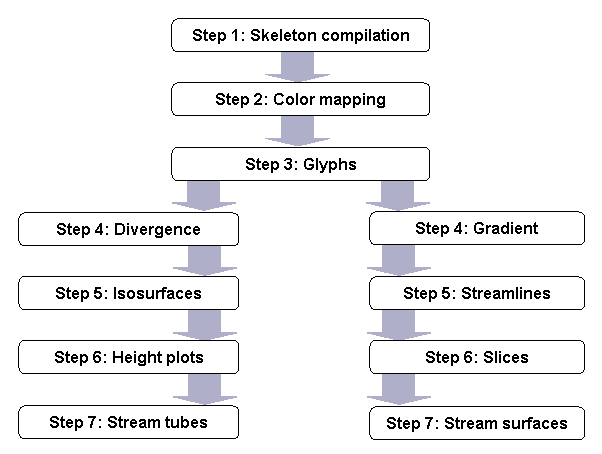
\includegraphics[scale=\imagescalefactor]{images/overview.png}
	\caption{The suggested workflow.}\label{fig:overview}
	\end{figure}

\chapter{Detailed description}\label{detaileddescription}
    \section{Architecture}
        This section describes the current architecture of our program. An overview of all the main components is given and the main functionality of each component is described. As can be seen in Figure \ref{fig:architecture}, our program consists of five main components.

        The \texttt{Smoke} class is the base class of the program, so the main functionality of this class is to visualize the simulated smoke. The simulation options, such as simulation speed, whether the smoke, vectors or iso lines should be drawn, are also implemented in this class.

        The \texttt{ColormapSelectPanel} class contains the basic functionality that is used for all the color maps that are used in our program. A color map for each data set ($\rho, |f|, |v|, div~f$ and $div~v$) can be chosen. Also, the scaling and clamping of colors from color maps can be enabled using the functionality in this class, the number of colors used in a color map can be specified and an appropriate type of color map can be selected. This class offers functionality that is used in a number of other classes that are used to specify color maps for different parts of our program.

        The \texttt{VectorOptionsSelectPanel} class enables the selection of a number of options of the vectors and glyphs that can be shown. Beside the functionality that was offered by the \texttt{ColormapSelectPanel} class, there are a number of other parameters that can be specified. The extended functionality consists of selecting the size of the vectors, the scale factor of the vectors and the number of grid points on which the vectors are drawn.

        The \texttt{IsoLineSelectPanel} class is also a descendent of the \texttt{ColormapSelectPanel} class. Besides all the functionality of this class, the number of iso lines and the values between which the iso lines are drawn can be chosen.

        The \texttt{HeightplotSelectPanel} class does not have all the functionality of the \texttt{ColormapSelectPanel} class. Selecting a color map was not useful here, so this functionality has been removed. However, shading and lighting options for the height map have been added.

		\begin{figure}[h]
		\centering
		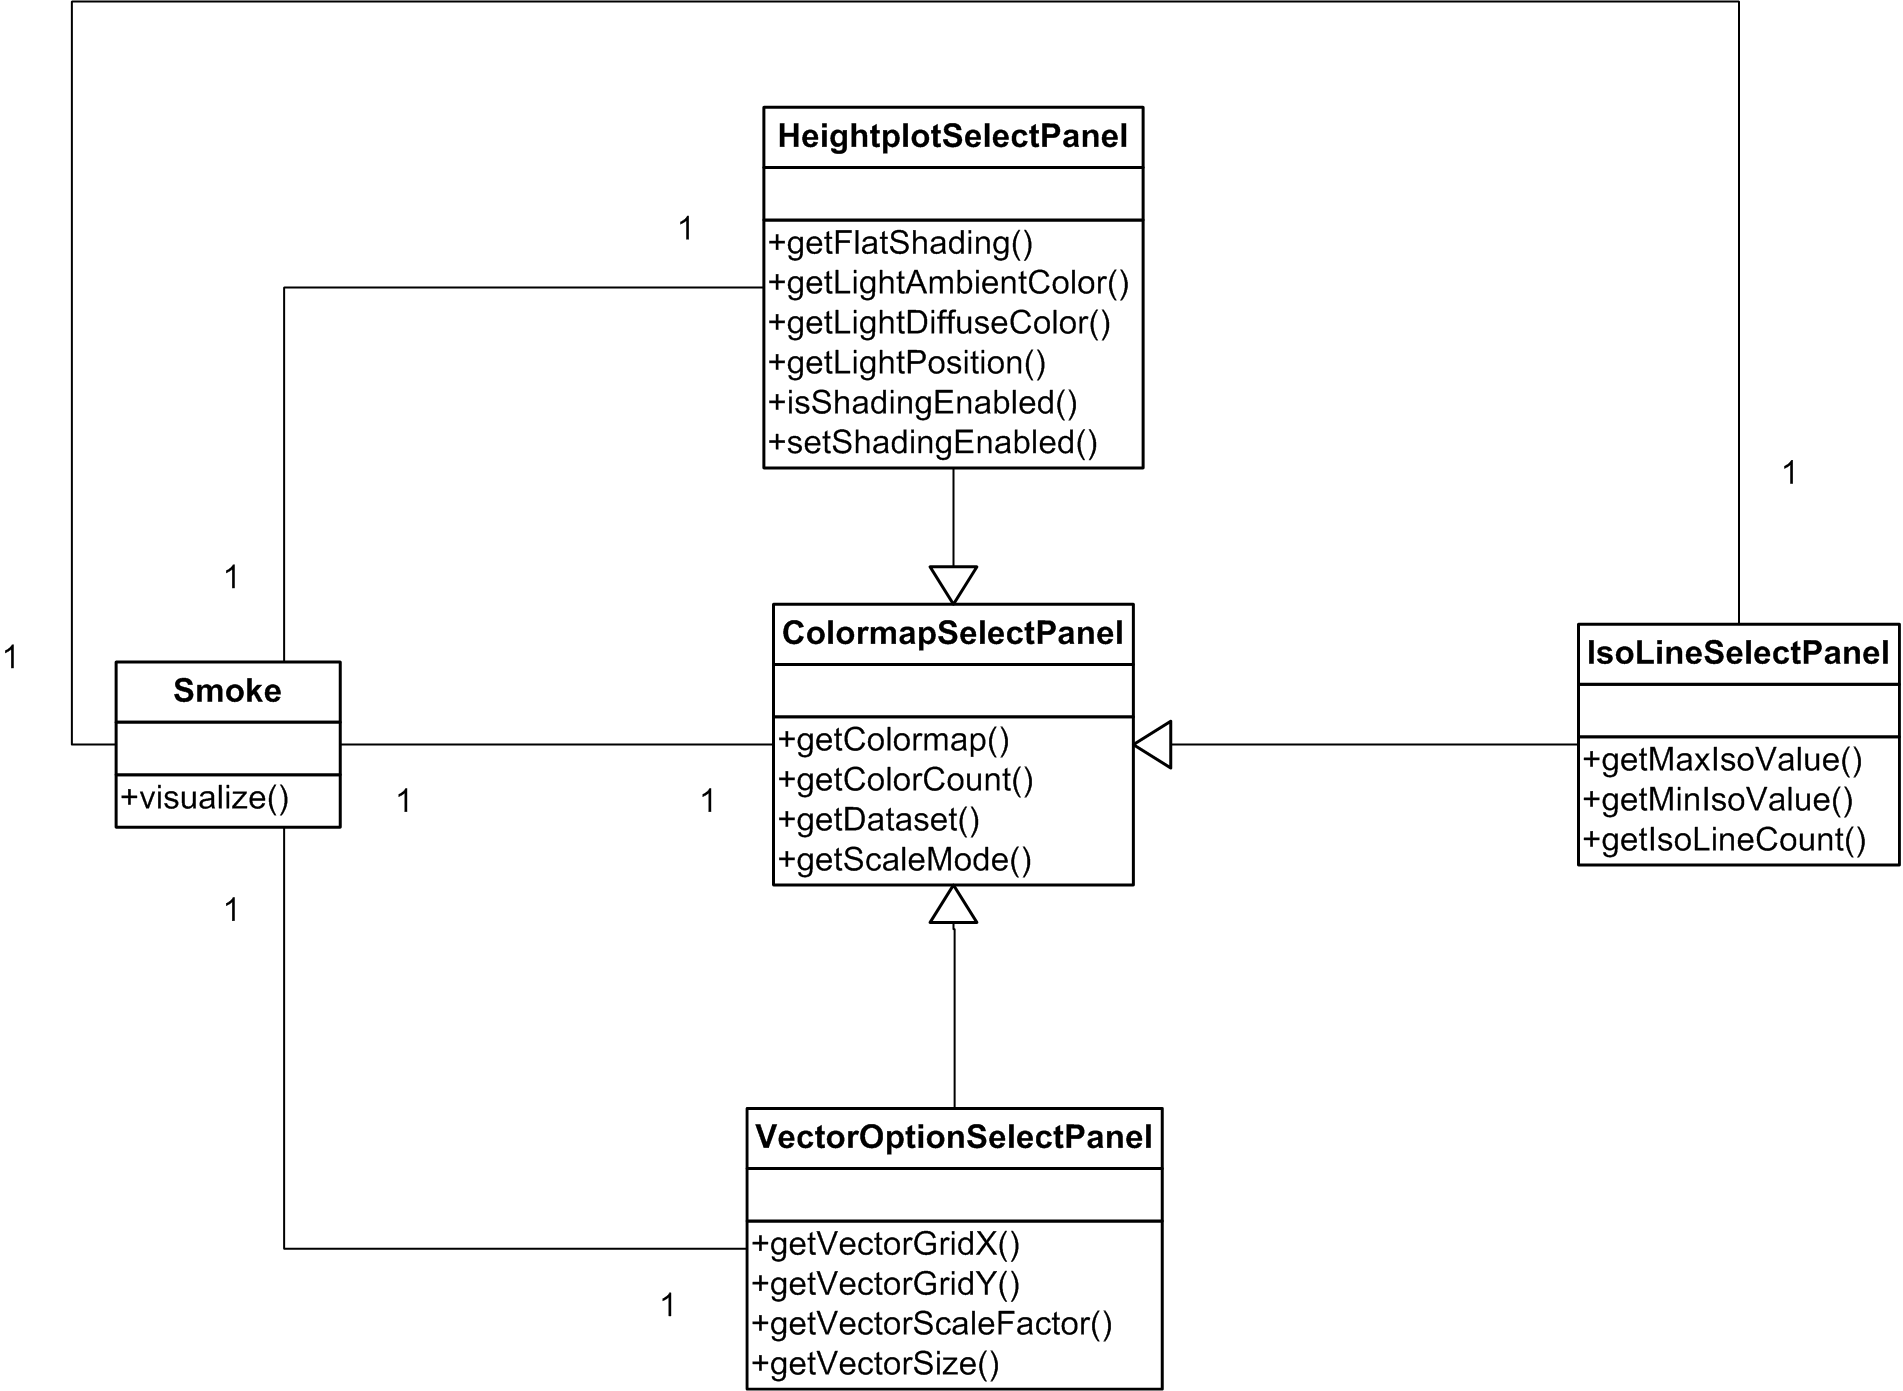
\includegraphics[scale=1.0]{images/architecture.png}
		\caption{The basic architecture of our program.}\label{fig:architecture}
		\end{figure}
		\clearpage
	\section{Skeleton compilation}
		This step does not really warrant much discussion. The only reasons to include it in our discussion here is to show what the program looked like when we first used it, and to point out one problem that we encountered at this point. The problems lies in an (in our opinion) flaw in the given source code, which uses an GLJPanel. The problem is that a GLJPanel is very slow, giving low framerates under Windows, and unacceptable framerates  under Linux. The solution we used was to simply replace the GLJPanel with a GLCanvas which is much faster. One problem with this approach was pointed out by dr.ir. H. van de Wetering which is that when embedding a GLCanvas in other Swing controls there may be some problems with the drawing of the visualization. However since we placed the Swing gui-elements next to the visualization windows we did not have any problems.
		\begin{figure}[h]
		\centering
		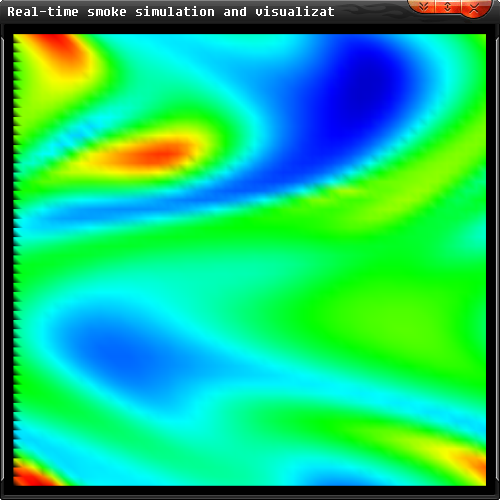
\includegraphics[scale=\imagescalefactor]{images/step1.png}
		\caption{The initial look of the program.}\label{fig:step1}
		\end{figure}
		\clearpage
	\section{Color mapping}
		The first real task was to set up a mechanism to implement color mapping. We choose to first do this as straight forward as possible and put all controls for the program on the same panel. In later versions of the program some of these controls would be put on a tab of their own. The dataset selection, scaling and clamping and colormapping boxes would later be factored into a reusable component.

		We have provided controls to select the dataset to visualize. Possible choices are density (rho or $\rho$) which indicates the density of the fluid simulation, force ($|$f$|$ or $|\overrightarrow{F}|$) which indicates the \emph{ammount} of force being applied at a certain point and velocity ($|$v$|$ or $\overrightarrow{v}$) which indicates the \emph{ammount} of movement of the fluid.

		It is also possibly to enable `scaling' and `clamping'. What scaling does is to scale sample-values that are read from the simulation to the range $[0..1]$. This is done by keeping track of the highest and lowest recorded sample-values in the previous frame, and using this to scale values read for the current frame. This makes the flow easier to see as the entire scale of the color-map will always be used, e.g. the highest peak will correspond to the high-end of the color-map and the lowest valley will correspond to the low-end of the color-map regardless of the actual values of those peaks and valleys.
		Clamping simply clamps the sample-values are read from the simulation to a user specifiably range. This means that the lowest possible value that can be read from the simulation is equal to the user-set lower bound, and similarly so for the highest possible value.
		Note that clamping is applied before scaling, allowing for the option to use the entire range of the color-map to visualize just a part of the sample-values generated by the simulation.

		Furthermore it is possible to specify a color-map to apply to the simulation. Three pre-defined colormaps are available, as well as one user definable colormap. The available predefined color-maps are a `rainbow' colormap which unsurprisingly consists of all colors present in a rainbow, a grayscale map where higher values are colored brighter, and a `Defined' map which is essentially the `rainbow' colormap with a limited number of gradient steps. For all of these color-maps it is possible to specify the number of steps in which the gradient should be divided by using a slider.
		A user can design his or her own favorite colormap by using the `Custom' setting. Colors can be added, changed or removed by right-clicking on a color and selecting the appropriate option. A minimum of at least two colors must be present, but no restriction is placed on the uniqueness of colors. Thus any gradient (even a single color) can be designed easily.

		One interesting feature that we added after seeing it in action on another groups visualization is the use of texture mapping for the application of the color-map to the simulation grid. To this end we construct a one-dimensional texture which holds the gradient that the user has selected and use the sample-values at the grid points as in texture coordinate into this texture. The advantage of this method over the use of simply specifying a color for each grid-point is best seen when the number of colors in the color-map is low. By specifying that the texture mapping algorithm should use `nearest-neighbour' interpolation over the polygon we obtain sharp edges along the color-bands, instead of the more blurred look that would otherwise be obtained. This better matches the definition of the color-map as is also visible in the preview window.

		Finally we applied one minor bug-fix; in the supplied Java code the left-most row of the grid shows some triangular artifacts (as can be seen in figure \ref{fig:step1}). This was caused by an improper initialization of some colors in the for-loop that draws the grid and easily solved.
		\begin{figure}[h]
		\centering
		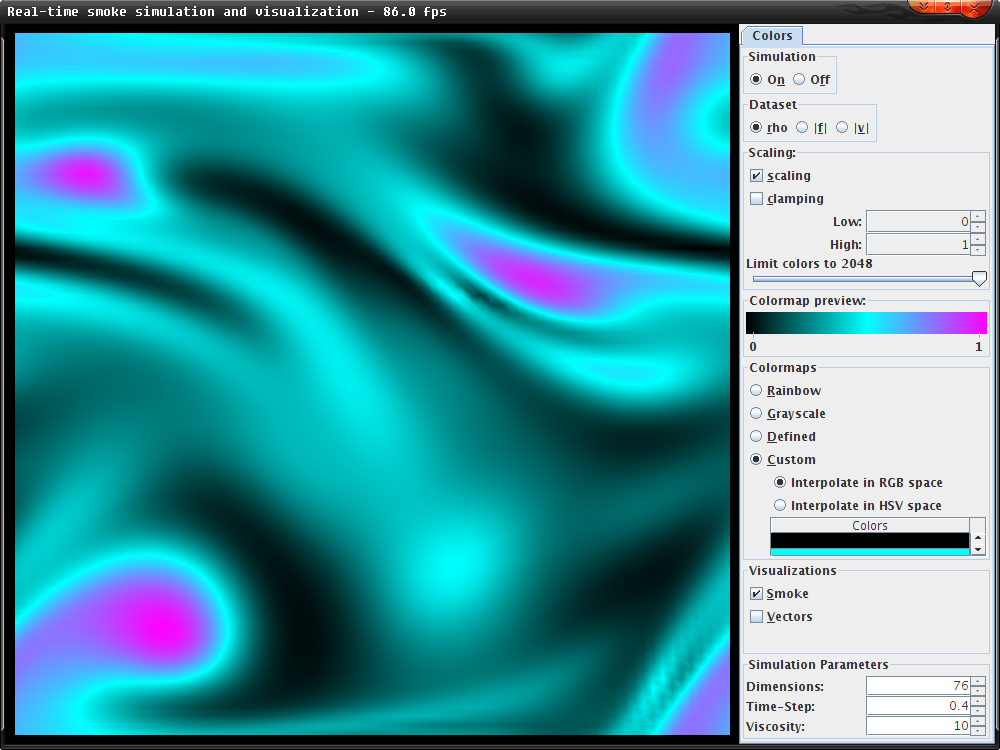
\includegraphics[scale=\imagescalefactor]{images/step2.png}
		\caption{The first gui elements.}\label{fig:step2}
		\end{figure}
		\clearpage
	\section{Glyphs}
		Next we implemented glyphs. As can be seen in the screenshot there are now three separate option panels. One panel can be used to set general options for the simulation (such as the size of the simulation grid, speed of simulation, etc.), one to set options for the `smoke', and one for the glyphs (vectors). The Vector panel in this screenshot is a specialization of the Smoke panel. The glyphs can be colored on any of the available datasets in the same way as the smoke.

		Also it is possibly to choose a different vector-field to align the glyphs with, and a different shape for the glyphs. The glyphs scale with the average magnitude of the sample-values around the glyph. This scaling can be influenced with the scale-factor to increase or decrease the sensitivity of the glyph scaling to the sample-values. The number of glyphs in the X- and Y-direction can also be set. A notable feature that we have implemented is that glyphs use the average sample values around them instead of just a single point value. This means that when there are significantly less glyphs than grid points glyphs will more more naturally with the flow (they respond to a larger area of the fluid-simulation, an area approximately the size of the glyph it self).
		Lastly it is also possible to select a different shape for the glyph, in the screenshot you can see the default `arrow' shape.
		\TODO{Andere shapes ook noemen? Welke 3D doen we dan?}
		\begin{figure}[h]
		\centering
		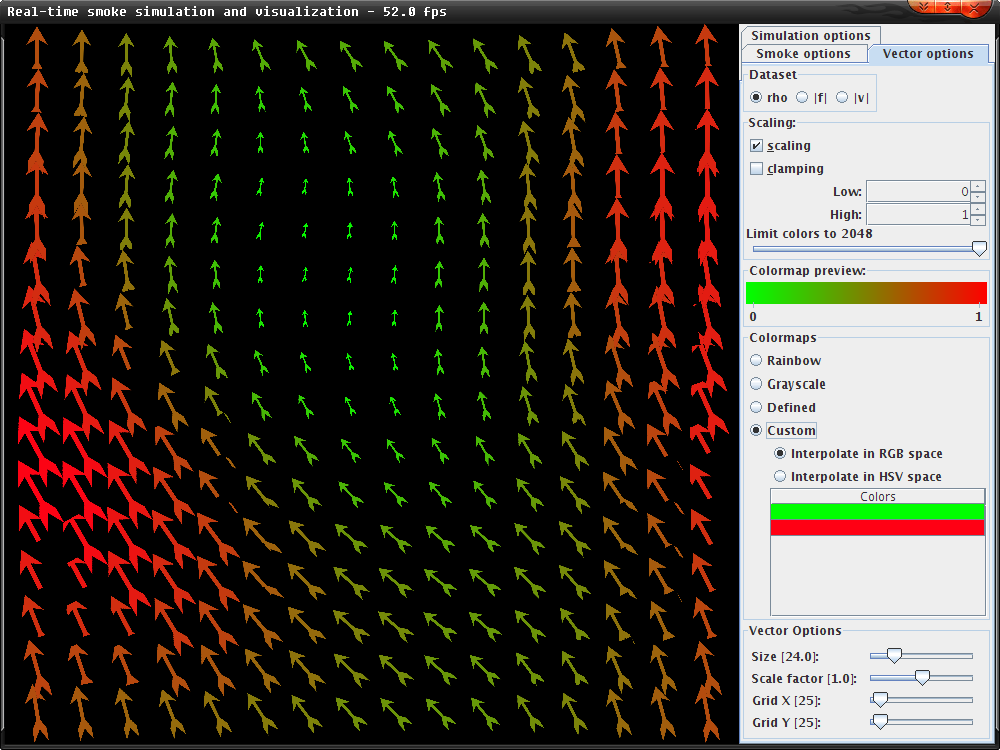
\includegraphics[scale=\imagescalefactor]{images/step3.png}
		\caption{Adding glyphs.}\label{fig:step3}
		\end{figure}
		\clearpage
	\section{Divergence}
        In the next stage of the assignment we implemented the possibility to view the divergence of $|v|$ and $|f|$. This was relatively easy, because the mechanism to select $div~v$ and $div~f$ had to be added in only one component of our program. The implementation of the value of these divergences on a grid point in our simulation was a little bit more complicated.

        The divergence $div~v$ is given by $div~v = \nabla \cdot v = \frac{\partial v_x}{\partial x} + \frac{\partial v_y}{\partial y}$ and the divergence of $|f|$ is $div~f = \nabla \cdot f = \frac{\partial f_x}{\partial x} + \frac{\partial f_y}{\partial y}$. To implement this, we had to determine the partial derivatives of $|f|$ and $|v|$. We have chosen to implement this by summing the values of respectively the data sets $|f|$ and $|v|$ around a grid point and take the mean of these sums.

        So put together in a formula, where $x$ and $y$ denote the coordinates of the grid points to determine $div~f$ or $div~v$: $div^*~v = \frac{1}{2}((v_{x-1,y} - v_{x+1,y}) + (v_{x,y-1} - v_{x,y+1}))$ and $div^*~f = \frac{1}{2}((f_{x-1,y} - f_{x+1,y}) + (f_{x,y-1} - f_{x,y+1}))$. Here $f_{x,y}$ and $v_{x,y}$ depict the values of respectively $f$ and $v$ on grid point $(x,y)$.   An example of the visualization of the divergence of $|v|$ is shown in Figure \ref{fig:step4}.
		\begin{figure}[h]
		\centering
		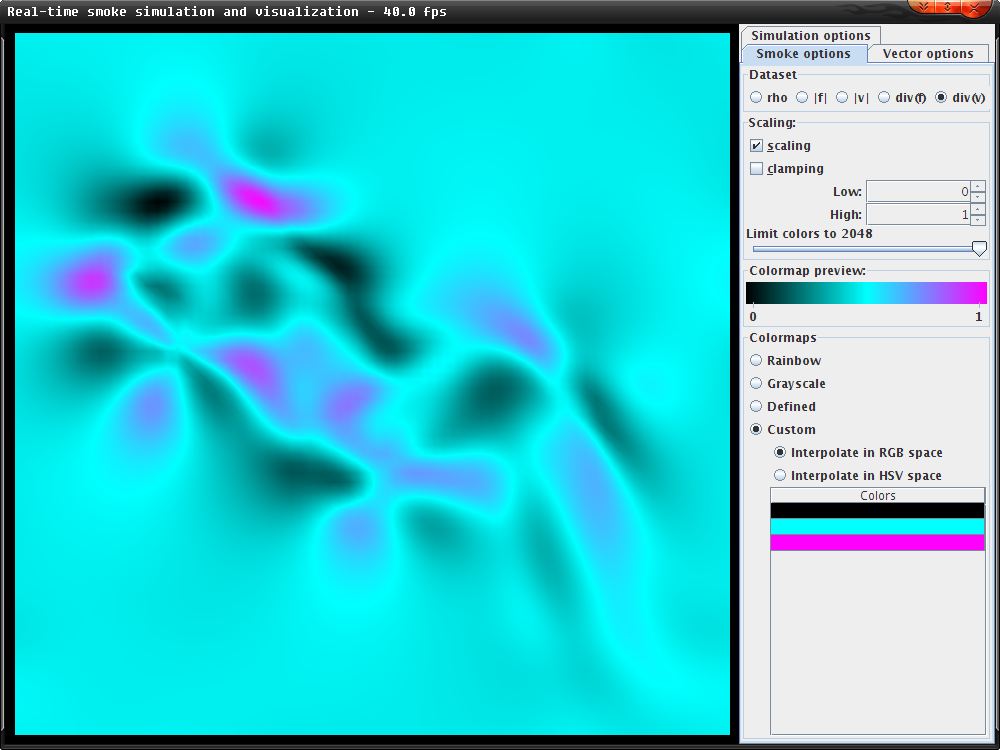
\includegraphics[scale=\imagescalefactor]{images/step4.png}
		\caption{Visualizing divergence.}\label{fig:step4}
		\end{figure}
		\clearpage
	\section{Isosurfaces (Isolines)}
        In this stage we had to implement the isoline technique. This part of the assignment consisted of two separate parts: adding functionality to place an isoline for one value of $\rho$, namely $\rho_0$ and placing a number of isolines between two values of $\rho$, being $\rho_1$ and $\rho_2$. We have chosen to generalize this part of the assignment. In our simulation it is not only possible to draw isolines only on values of $\rho$, but also on $|v|, |f|, div~v$ and $div~f$.
        
        As can bee seen in Figure \ref{fig:step5} a new tab with properties for the isolines was added. Here (amongst color and data set options) $\rho_1$(Low) and $\rho_2$(High) and the number of iso lines that should be drawn between these two can be specified. If $\rho_1 = \rho_2$, only one iso line is drawn. In our visualization this is the way to select a $\rho_0$.
        
        Our isolines are constructed from a number of partial isolines. These partial isolines together form a closed isoline. We use a lookup table to determine how a partial isoline should be drawn.
		\begin{figure}[h]
		\centering
		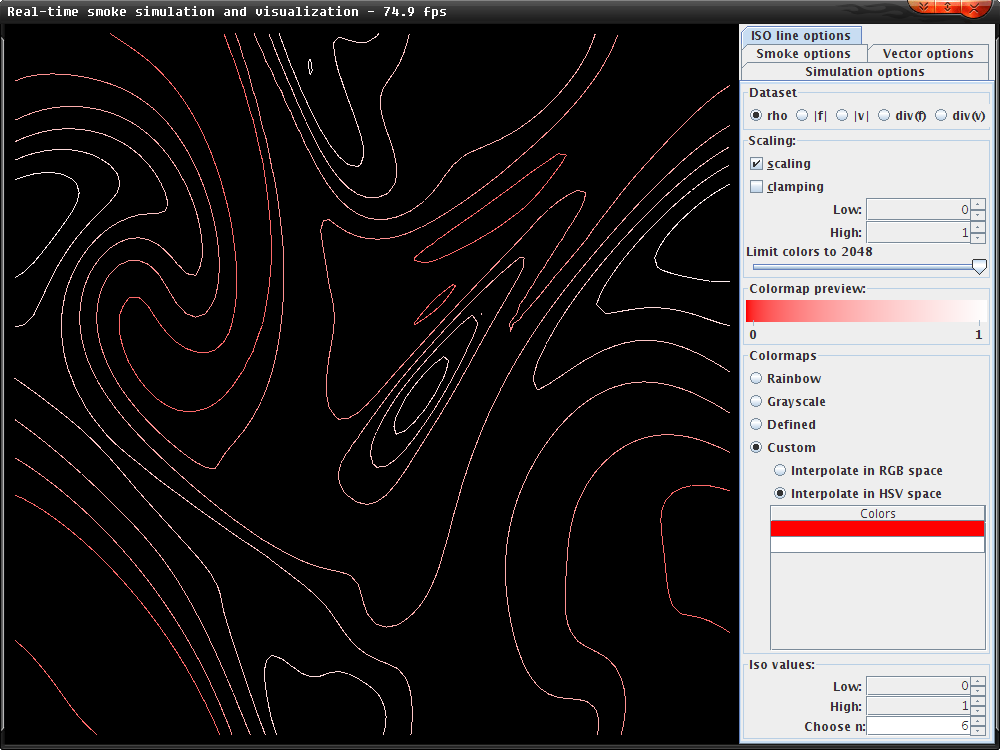
\includegraphics[scale=\imagescalefactor]{images/step5.png}
		\caption{Drawing isolines.}\label{fig:step5}
		\end{figure}
		\clearpage
	\section{Height plots}
		In this step the visualisation was transformed from a 2-dimensional view to a 3-dimensional view. This step was surprisingly easy, as we had first thought it would involve a lot of work. It turned out to be mostly a matter of building the options-panel where the user can set the options for the heightplot, and replacing the 2-dimensional drawing calls to OpenGL with 3-dimensional ones, using the heightplot's sample-values for the Z-coordinate.

		We assumed that the goal of this assignment was to transform the actual 2-dimensional simulation-grid into a 3-dimensional grid. This was based on the description on the assignment-website which stated `That is, use the already existing simulation grid geometry as base plane for the height plot.' and further motivated by the the following arguments. Firstly it was our opinion that having a separate heightplot above or below the 2-dimensional smoke does not provide a better view of the simulation, and instead often obscures the view of one of the two. Secondly implementing the heightplot as a separate grid would double the ammount of geometry being drawn in a single frame, effectively cutting the framerate almost in half. This, combined with the fact that the framerate of our application had already dropped considerably over the course of adding more and more features we opted to implement the heightplot straight into the existing visualisation.

		In order to help fend against misinterpretation of the visualisation data due to the effects of perspective, the 3-dimensional view is drawn in isometric view. Thus a glyph with appears to be smaller than some other glyph also actually \emph{is} smaller than that other glyph. This has the added bonus that when the visualisation is viewed from straight above, it appears exactly the same as the 2-dimensional simulation would.
		\begin{figure}[H]
		\centering
		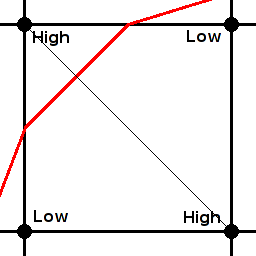
\includegraphics[scale=\imagescalefactor]{images/isolinetrouble.png}
		\caption{Example of an isoline crossing geometry.}\label{fig:isolinetrouble}
		\end{figure}
		Some minor issues were encountered, first of which is that the geometry of the simulation-grid and isolines would often `clip', that is parts of the isolines would intersect with the simulation-grid since they do not share the same grid-points (a section of an isoline can have start- and end-point half-way between two grid points). (See figure \ref{fig:isolinetrouble} for an example; here two opposite grid points have a high resp. low value, and the isoline has a value inbetween. because the grid is constructed from triangles such that they have a common edge on the line from high to high the isoline will go through the geometry). This caused noticeable breaks in the isolines. We tried several solutions including drawing thicker lines, but the solution that worked best was to draw the isoline slightly higher than the point where it is supposed to be drawn, thus raising it slightly above the geometry of the heightplot.
		Secondly there is a similar problem with the glyphs. Fortunately it is not as visible as in the case of the isolines, so we did not bother to correct the issue in this case. One nice addition which we unfortunately could not easily implement would be to draw the glyphs along the slope of the smoke geometry, thus raising and lower the tips of the glyphs in accordance with the underlying landscape.

		The following controls were provided; the usual dataset and scaling/clamping options, an option to turn on or off the lighting model, the ability to select the diffuse and ambient color of the light source, a choice between either `flat' shading or `smooth' shading and a rudimentary position selection for the light-source. To use the light-source position selector first imagine a color-cube. That is a cube such that the horizontal x-axis has red values increasing to the left, the y-axis has blue increasing to the lower right and the vertical z-axis as green increasing towards the top. Now imagine the scene at the center of the cube. Now the color you pick represents the position of the light.
		The orientation of the camera is controlled by dragging with the right-mousebutton in the simulation field. The view can be reset to the default top-down view by pressing the middle-mousebutton.
		\begin{figure}[h]
		\centering
		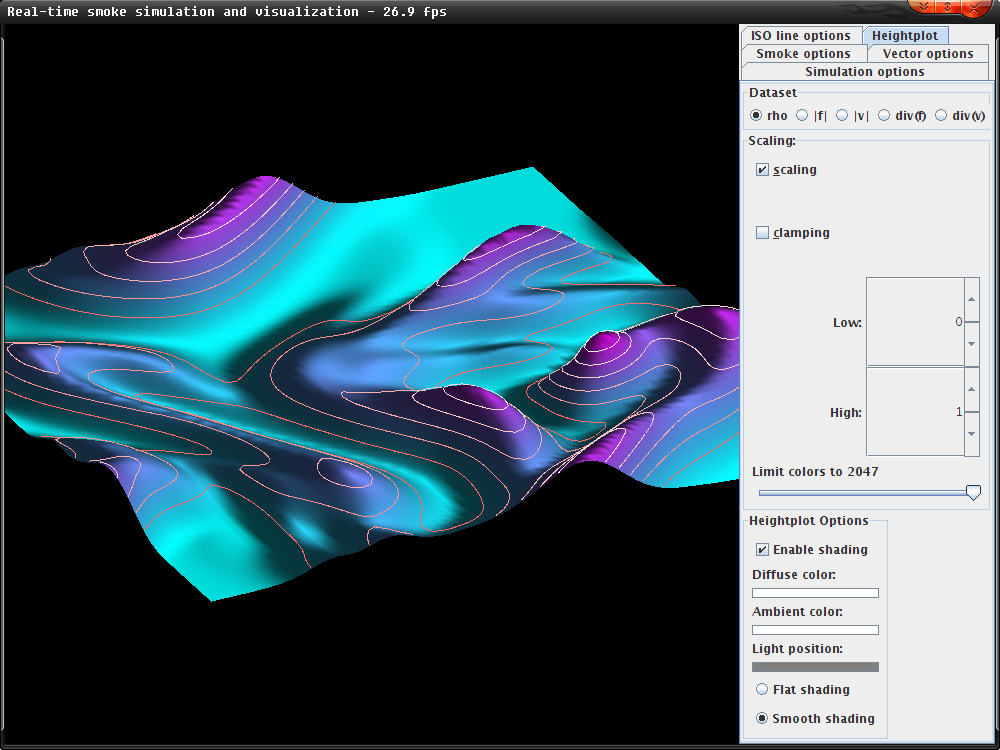
\includegraphics[scale=\imagescalefactor]{images/step6.png}
		\caption{The heightplot.}\label{fig:step6}
		\end{figure}
		\clearpage
	\section{Stream tubes}
		The final step in the development of the program is adding a visualization using stream tubes. Unfortunately this part of the program is still under development at the time of writing, and as such we can not provide a screenshot at this time. We do hope to have completed implementation of stream tubes before the final presentation.
		Since we do not yet have a working stream tube implementation we also do not yet have an interface for controlling the visualization. We can however describe the controls that we plan to implement, and a possible approach that we could take. The controls that we need to implement are the selection of a scalar field for use a the diameter. We can reuse part of our SelectPanels for this, allowing users to also scale and clamp the sample-values. We also need a method to allow users to place the seed-points. For this we could consider a two-step technique where a user first clicks somewhere inside the visualization window to place a seed-point, upon which a seed point is placed and marked. Next the user can use the mousewheel to change the depth of the seed point.

		For the actual implementation of the stream tubes the most challenging part will be the actual construction of the stream tube's geometry. Obtaining the 3-dimensional dataset is fairly easy as it simply involves keeping the last $N$ datasets arrays, which can simply be achieved by placing the current dataset arrays in an encompassing array, and generating new dataset arrays and deleting the oldest dataset arrays every frame. From here on tracing a stream line should be possible be using a similar technique as in step 5b, but in 3-dimensions. It might be possible to construct and output the geometry for the stream tube as the stream line is traced.

		Finally we need to look at where exactly in the current visualization we will place the stream tubes, as they might interfere with the heightplot. One solution might be to force the user to choose between either a heightplot or stream tubes.
\chapter{Conclusion}
% klein stukje slap gezever
\end{document}
